\documentclass[a4paper,twoside,12pt,hidelinks]{article}

% Packages
% ---------------------

% \usepackage{amsmath} % Needed for command eqref
\usepackage{amsthm} % Used to show the proof box
\usepackage{fancyhdr} % Head and foot options
\usepackage{hyperref} % Uses automatic references \autoref
\usepackage{titletoc} % Style table of contents with dots
\usepackage[T1]{fontenc}
\usepackage{libertine}
\usepackage{multirow}
\usepackage[libertine]{newtxmath} % Font
% \usepackage{pgfplots} % Drawing graphsrestrict y to domain=-20:20
\usepackage{empheq} % draw box around multiple align equations
\usepackage{float} % Forcing text after image https://stackoverflow.com/a/2828029/297131
% \usepackage{breakcites} % Break long citations into separate lines
% \usepackage{physics} % Used for vector component notation
% \usepackage{mathtools} % Used for vector component notation
\usepackage{siunitx} % Physical numbers and units
\usepackage{bm} % Used for vector component notation
% \usepackage[makeroom]{cancel} % for using \cancel{...}
% \usepackage[tableposition=top]{caption} % Place captions on top of the tables
\usepackage{listings} % Source code
% \usepackage[bottom]{footmisc}
% \usepackage{tocloft} % Reduce space between line in the table of contents
% \usepackage{soul} % For strike through text \st{cow}
% \usepackage{enumitem} % reduce the separation in lists \begin{enumerate}[topsep=0pt] https://tex.stackexchange.com/a/86055
% \usepackage[most]{tcolorbox} % for putting frames around the text \begin{myframe}[width=\linewidth]
% \usepackage{natbib}
\usepackage{enumitem} % lists
\usepackage{array} % For making array column the same width https://tex.stackexchange.com/a/162847


% Page settings
% ---------------------

\usepackage[top=2cm, bottom=2.5cm,left=2.5cm,right=2.5cm]{geometry} %  Page margins
\setlength{\parskip}{\baselineskip} % Add space between paragraphs
\setlength{\intextsep}{20pt plus 2.0pt minus 2.0pt} % Add vertical space before and after tables and figures (http://tex.stackexchange.com/a/26522/101976)
\parindent=0cm % Remove the paragraph indent of the first line
% \setlength\cftparskip{4pt} % Reduce space between line in the table of contents
\addtolength{\jot}{2\jot} % Double the line between equations
\def\arraystretch{1.5} % Increase the vertical table cell margin
\dottedcontents{part}[0em]{\bfseries}{0em}{1pc} % Use dots in the table of contents
\dottedcontents{section}[5em]{}{3em}{1pc} % Use dots in the table of contents
\renewcommand{\contentsname}{\centering Contents} % Center the table of contents header
\raggedbottom % Prevents spreading the page content vetically for non-full pages.
\setlength{\headheight}{20pt} % Height of the header
% \pgfplotsset{compat=1.12}
% \lstset{aboveskip=10pt,belowskip=-5pt} % space around code listing

% Set vertical space around equations.
\AtBeginDocument{%
 \abovedisplayskip=15pt plus 5pt minus 5pt
 \abovedisplayshortskip=12pt plus 3pt
 \belowdisplayskip=15pt plus 5pt minus 5pt
 \belowdisplayshortskip=12pt plus 3pt minus 4pt
}

\lstset{ %
language=Fortran,           % choose the language of the code
basicstyle=\footnotesize    % the size of the fonts that are used for the line-numbers
}

% Make the proof white box a black box.
% \renewcommand{\qedsymbol}{\rule{0.7em}{0.7em}}

% Show black box on the right
\newcommand{\myproof}{
  {
    \begin{flushright}
      \qedsymbol
    \end{flushright}
  }
}

% Draw circles around letters:
% \encircle{d}
% https://tex.stackexchange.com/a/123926
\usepackage{tikz}
\newcommand\encircle[1]{%
  \tikz[baseline=(X.base)] 
    \node (X) [draw, shape=circle, inner sep=0] {\strut #1};}

% For making array column the same width https://tex.stackexchange.com/a/162847
\newcolumntype{C}[1]{>{\centering\arraybackslash$}m{#1}<{$}}

\newcommand{\STAB}[1]{\begin{tabular}{@{}c@{}}#1\end{tabular}}

\newcommand{\largeletter}[1]{\text{\Large\ensuremath #1}}

\newcommand*\widefbox[1]{\fbox{\hspace{2em}#1\hspace{2em}}}

% PDFPlots
% Horizontal asymptote
%   Usage:
%     \begin{axis}[hasymptote=1]
% \pgfplotsset{hasymptote/.style={
%     before end axis/.append code={
%         \draw[densely dashed] ({axis cs:0,#1} -| {rel axis cs:0,0})
%         -- ({axis cs:0,#1} -| {rel axis cs:1,0});
%     }
% }}

% \tikzstyle{dashdotted}=[dash pattern=on 3pt off 2pt on \the\pgflinewidth off 2pt]

% \usepgfplotslibrary{fillbetween} % Fill area between graphs
% \usetikzlibrary{patterns} % Fill with pattern


\newenvironment{changemargin}[2]{%
\begin{list}{}{%
\setlength{\topsep}{0pt}%
\setlength{\leftmargin}{#1}%
\setlength{\rightmargin}{#2}%
\setlength{\listparindent}{\parindent}%
\setlength{\itemindent}{\parindent}%
\setlength{\parsep}{\parskip}%
}%
\item[]}{\end{list}}


% Column vector: \myvec{x\\y\\z}
% Row vector: \myvec{a&b&c}
\newcommand{\myvec}[1]{\ensuremath{\renewcommand*{\arraystretch}{0.9}\begin{bmatrix}#1\end{bmatrix}}}

% Use to draw vertical line in bmatrix
% https://tex.stackexchange.com/a/299241/101976
\newcommand\aug{\fboxsep=-\fboxrule\!\!\!\fbox{\strut}\!\!\!}

% \lstset{ %
% language=Mathematica,           % choose the language of the code
% basicstyle=\footnotesize    % the size of the fonts that are used for the line-numbers
% }


% For puttin frames around the text \begin{myframe}[width=\linewidth]
% \newtcolorbox{myframe}[1][]{
%   enhanced,
%   arc=0pt,
%   outer arc=0pt,
%   colback=white,
%   boxrule=0.8pt,
%   top=10pt,
%   bottom=13pt,
%   left=0pt,
%   right=20pt,
%   arc=10pt,
%   auto outer arc,
%   #1
% }

\def\code#1{\texttt{\small#1}} % Format code inlint \code{myFunction}

% Title page

\title{Fortran program for root estimation using Newton-Raphson method}
\author{Written by Evgenii Neumerzhitckii}
\date{Aug 9, 2019}

\begin{document}

\setcounter{secnumdepth}{-1}
\renewcommand{\thepart}{}
\renewcommand{\thesection}{Part \Alph{section}}
\renewcommand{\thesubsection}{\Alph{section}.\arabic{subsection}}
\renewcommand{\partname}{}


\maketitle
\thispagestyle{empty} % Remove page number from title page
% \vspace{3.5cm} % Add space between the title and table of contents
% \tableofcontents
% \thispagestyle{empty} % Remove page number from title page

% \pagebreak
\pagebreak


% Header and footer
% ---------------------

\pagestyle{fancy}
\fancyhf{}
\fancyhead[C]{ASP3162}
\renewcommand{\headrulewidth}{0.1pt}
\cfoot{\thepage}


% Parts
% ---------------------

% \input{parts/quote}
% \pagebreak

% \input{parts/summary}
% \pagebreak

\section{The advection equation}

In want to solve the following advection equation
\begin{equation}
  v_t + v v_x = 0,
  \label{eq_advection}
\end{equation}
where $v$ is velocity, $t$ is time, $x$ position, and $v_t$ is a short notation for the derivative $\frac{\partial v}{\partial t}$. We have the following initial condition
\[
  v(x, 0) = \cos x,
\]
and we want to solve the equation for values of $x$ and $t$ from the intervals
\begin{equation}
  -\pi < x < \pi, \quad \quad 0 \leq t \leq 1.4.
  \label{eq_x_t_ranges}
\end{equation}


\section{Using analytical solution}

Here we use analytical solution of \autoref{eq_advection}:
\begin{equation}
  v = \cos (x - v t ).
  \label{eq_analytical_solution}
\end{equation}
Our goal is to write a Fortran program that solves \autoref{eq_analytical_solution} for various values of $x$ and $t$ parameters from the intervals given by Inequalities \ref{eq_x_t_ranges}.

\subsection{Using Newton-Raphson method}

In order to solve \autoref{eq_analytical_solution} numerically, we use Newton-Raphson method:
\begin{equation}
  v_{n+1} = v_n - f(v_n, x, t) / f'(v_n, x, t),
  \label{eq_recurrence}
\end{equation}
where $n=1, 2, \dots, N_{max}$ is the iteration number with $N_{max}$ being the maximum number of iterations, and
\[
  f(v_n, x, t) = \cos (x - v_n t) - v_n,
\]
which is constructed by moving the terms of \autoref{eq_analytical_solution} to one side. Here $x$ and $t$ are fixed values that do not change during this calculation.

We begin the calculations by choosing a starting $v_1$ value and then use \autoref{eq_recurrence} to calculate $v_2$. Then we use $v_2$ to calculate $v_3$. This calculation is repeated until the absolute difference between two subsequent $v$ values is smaller than a chosen tolerance number $\epsilon$:
\[
  |{v_{n+1} - v_n}| < \epsilon.
\]
The calculations are also stopped and the program is terminated with an error if the number of iterations exceeds a chosen maximum number of iterations $N_{max}$. The program is also terminated if devision by zero or an overflow is detected as a result of calculating $v_{n+1}$ from \autoref{eq_recurrence}.

\subsection{Finding roots for different values of $x$ and $t$}

Our goal is to find roots of \autoref{eq_analytical_solution} for different values of $x$ and $t$ from the intervals defined by Inequalities \ref{eq_x_t_ranges}. In order to calculate these roots, we use Newton-Raphson method multiple times by choosing values of $x$ and $t$ from the following sequences:
\begin{align*}
  \{ x_{\textrm{start}}, x_{\textrm{start}} + \Delta x, x_{\textrm{start}} + 2 \Delta x, \dots, x_{\textrm{end}} \} \\
  \{ t_{\textrm{start}}, t_{\textrm{start}} + \Delta t, t_{\textrm{start}} + 2 \Delta t, \dots, t_{\textrm{end}} \},
\end{align*}
where $x_{\textrm{start}}$, $x_{\textrm{end}}$ are the smallest and largest $x$ values, and $t_{\textrm{start}}$, $t_{\textrm{end}}$ are the smallest and largest $t$ values that are supplied to the program by the user The values $\Delta x$, $\Delta t$ are the position and time steps that are calculated as follows:
\begin{align}
  \Delta x &= \frac{x_{\textrm{end}} - x_{\textrm{start}}}{n_x - 1} \label{eq_dx} \\
  \Delta t &= \frac{t_{\textrm{end}} - t_{\textrm{start}}}{n_t - 1}, \label{eq_dt}
\end{align}
where $n_x$ and $n_t$ are the number of position and time steps that are supplied to the program by the user.


\subsection{Writing the code}

Next, we write Fortran code to solve \autoref{eq_analytical_solution}. The code shown in \autoref{code_solve_v_equation} is a part of \code{find\_many\_roots} function. The code calculates the roots of \autoref{eq_analytical_solution} for various values of $x$ and $t$ parameters.

\noindent\begin{minipage}{\linewidth}
\begin{lstlisting}[caption={Solving $v = \cos (x - v t )$ equation for various values of parameters $x$ and $t$ (\code{root\_finder.f90}).},frame=tlrb,label={code_solve_v_equation}, numbers=left, firstnumber=160]
! Assign evenly spaced x and t values
call linspace(x_start, x_end, x_points)
call linspace(t_start, t_end, t_points)

! Calculate step sizes
dx = (x_end - x_start) / (nx - 1)
dt = (t_end - t_start) / (nt - 1)

! Calculate solutions for all values of x and t
do it = 1, nt
    do ix = 1, nx
        x = x_start + (ix - 1) * dx
        t = t_start + (it - 1) * dt

        root = find_root(options=options, x=x, t=t, success=success)

        if (.not. success) then
            ! Could not find root: return the problematic x and t
            error_x = x
            error_t = t
            return
        end if

        solution(ix, it) = root
    end do
end do
\end{lstlisting}
\end{minipage}

On \code{Line 161} we assign evenly spaced values between $x\_start$ and $x\_end$ for the $x$-coordinate and store then in the \code{x\_points} array. The values \code{x\_start} and \code{x\_end}. The number of points $nx$ are also supplied to the program by the user and they determine the size of the \code{x\_points} array.

On \code{Line 162} use the same technique to calculate the values of the $t$-coordinate and store them in $\code{t\_points}$ array.

On \code{Lines 165} and \code{166} we calculate the position and time steps $dx$ and $dt$ using Equations \ref{eq_dx} and \ref{eq_dt}.

Next, on \code{Lines 169} and \code{170} we use two loops to iterate over the range of indexes $it$ and $ix$. Inside the loops, on \code{Lines 171} and \code{172} we calculate the values of the $x$ and $t$ parameters for the current iteration.

On \code{Line 174} we call \code{find\_root} function. This function calculates a root of \autoref{eq_analytical_solution} using Newton-Raphson method and returns this root.

Newton-Raphson method does not guarantee to find a root. The case when the program does not find a root is handled on \code{Lines 176-181}. Here we store the problematic values of $x$ and $t$ and exit the subroutine with an error.

Alternatively, in case when the program does find a root, we store that value in a 2D array called \code{solution} on \code{Line 183}.

The end result of this part of the program is the $\code{solution}$ array filled with values of $v$ for all values of $x$ and $t$ parameters that the user has chosen. Alternatively, if the program could not find solution to \autoref{eq_analytical_solution} for just a single pair of $x$ and $t$, it exits with an error. In this case, the user is presented with an error message containing the values of $x$ and $t$ parameters for which Newton-Raphson method failed. The user can then re-run the program again with different values of starting $v_1$ value, tolerance and maximum number of iterations $N_{max}$ for Newton-Raphson method, until she finds settings for which Newton-Raphson is able to find solutions for all values of $x$ and $t$.



\subsection{Running the program and making plots}

The source code is located in \code{01\_root\_finder} directory. Instructions for compiling, running the program and plotting its results are located in the README.md file that comes with the source code.


\subsection{Plotting solution}

We plot the output of our program \autoref{fig_solution_3d}.
\begin{figure}[H]
  \centering
  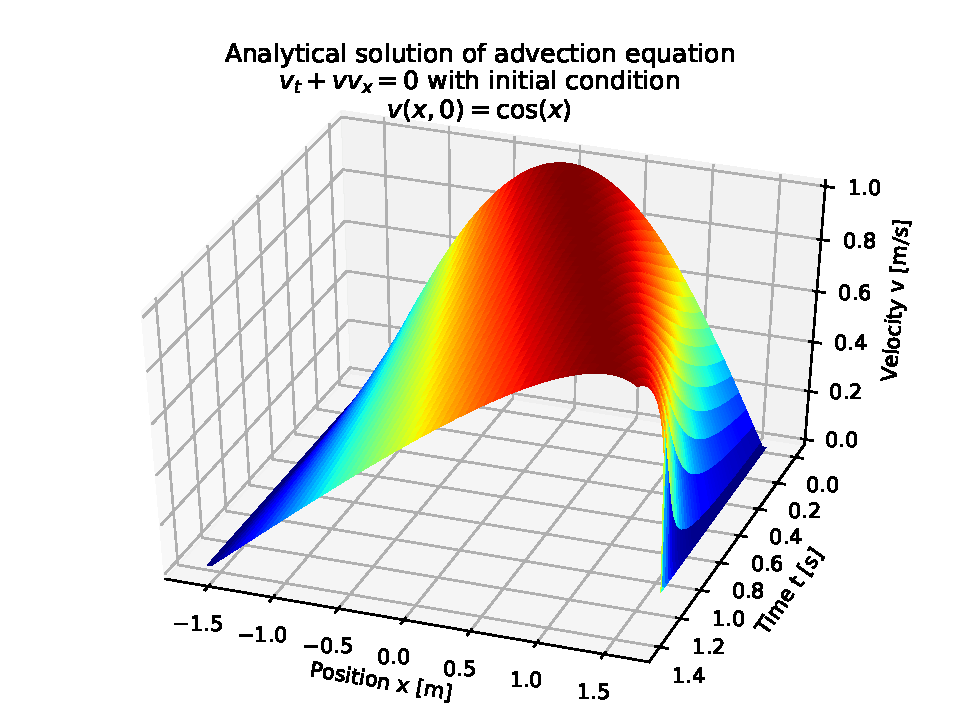
\includegraphics[width=1.0\textwidth]{figures/advection_analytical_solution_3d.pdf}
  \caption{Analytical solution of advection equation.}
  \label{fig_solution_3d}
\end{figure}
The 2D plot of the solution is shown on \autoref{fig_solution_2d}. We can see that as time increases, the solution curve becomes skewed to the right. After about $t > 1.2 s$, the right side of the curve becomes almost vertical, breaks and does not reach the zero value.
\begin{figure}[H]
  \centering
  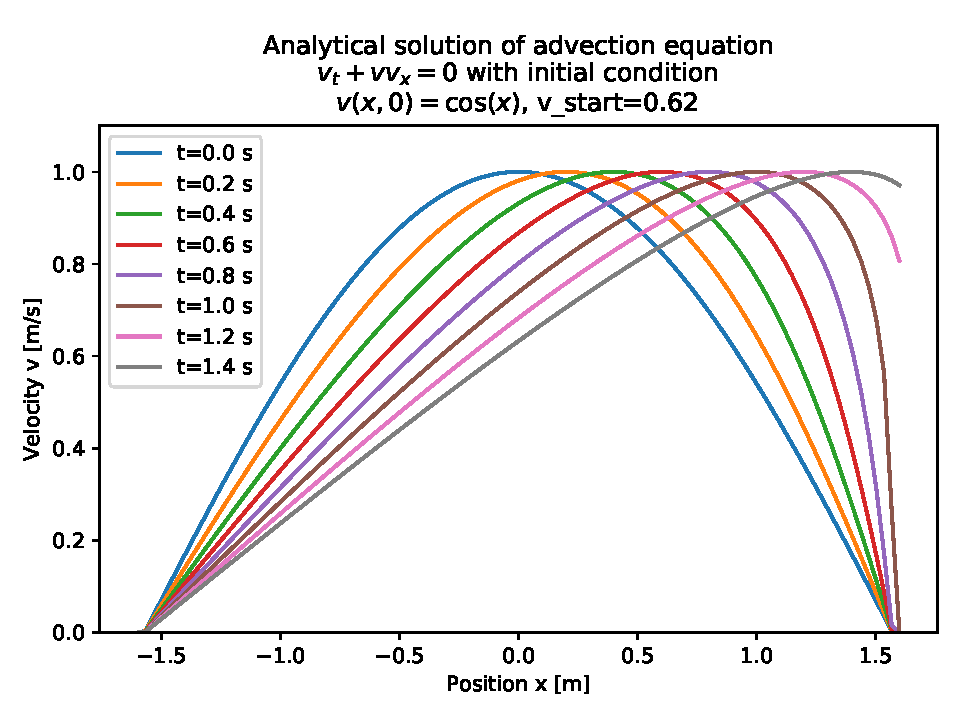
\includegraphics[width=1.0\textwidth]{figures/advection_analytical_solution_2d_vstart_0_62.pdf}
  \caption{Analytical solution of advection equation for various time values. The solution was calculated using \code{v\_start}=0.62 parameter for Newton-Raphson method.}
  \label{fig_solution_2d}
\end{figure}
In order to investigate the solution at high values of $t$ we run the program with different values of \code{v\_start} parameter (the initial value used for Newton-Raphson method), chosen between $0$ and $1$ We have found that Newton-Raphson method was not able to find a solution for most values $\code{v\_start} < 0.4$. In contrast, the program was able to find solutions for values $\code{v\_start} > 0.5$, especially those near $\code{v\_start} = 0.8$.

In addition, we have found that the choise of $\code{v\_start}$ affected the solution for $t > 1.2$. For example, using solutions for $\code{v\_start}=0.15$ are shown in \autoref{fig_solution_2d_0_15}.
\begin{figure}[H]
  \centering
  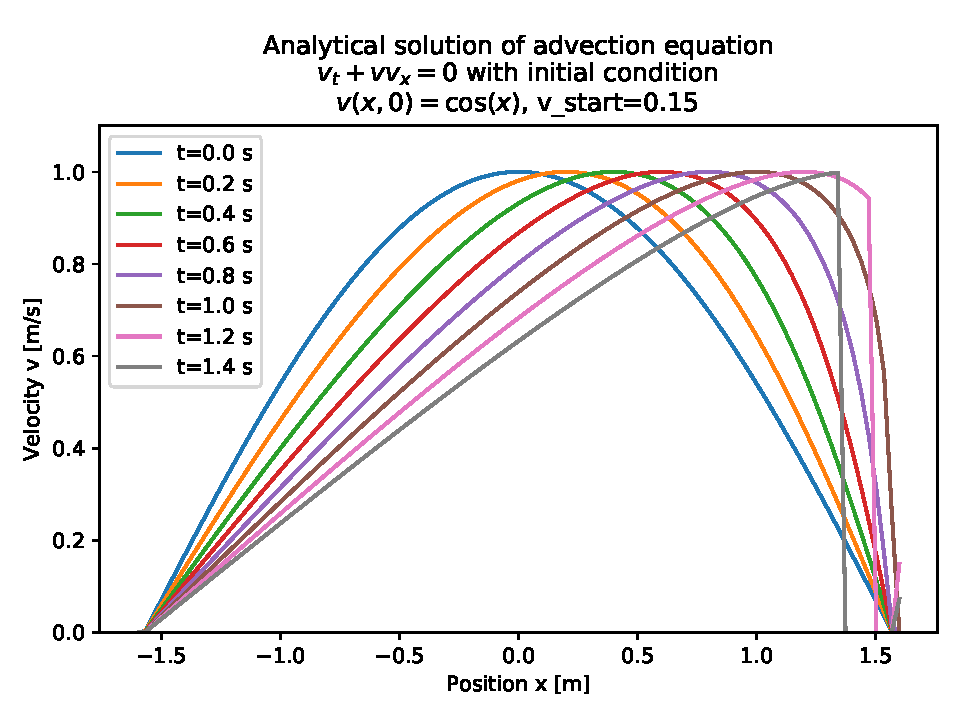
\includegraphics[width=1.0\textwidth]{figures/advection_analytical_solution_2d_vstart_0_15.pdf}
  \caption{Analytical solution of advection equation for various time values. The solution was calculated using \code{v\_start}=0.15 parameter for Newton-Raphson method.}
  \label{fig_solution_2d_0_15}
\end{figure}
\pagebreak

% \section{Task 2}

Hi there :)

% \pagebreak

% \part{Task 3}

The changes of mass fraction over time for a range of tempearures are shown on Figures \ref{fig_3.1_mass_fractions_t9_1.0} - \ref{fig_3.1_mass_fractions_t9_1.9}.

\begin{figure}[!ht]
    \centering
    \includegraphics[width=0.85\textwidth]{figures/{03.1_t9_1.0}.pdf}
    \vspace*{-5mm}
    \caption{Changes of mass fraction over time for temperature $T=\SI{1e9}{K}$.}
    \label{fig_3.1_mass_fractions_t9_1.0}
\end{figure}

\begin{figure}[!ht]
    \centering
    \includegraphics[width=0.85\textwidth]{figures/{03.1_t9_1.1}.pdf}
    \vspace*{-5mm}
    \caption{Changes of mass fraction over time for temperature $T=\SI{1.1e9}{K}$.}
    \label{fig_3.1_mass_fractions_t9_1.1}
\end{figure}

\begin{figure}[!ht]
    \centering
    \includegraphics[width=0.85\textwidth]{figures/{03.1_t9_1.2}.pdf}
    \vspace*{-5mm}
    \caption{Changes of mass fraction over time for temperature $T=\SI{1.2e9}{K}$.}
    \label{fig_3.1_mass_fractions_t9_1.2}
\end{figure}

\begin{figure}[!ht]
    \centering
    \includegraphics[width=0.85\textwidth]{figures/{03.1_t9_1.3}.pdf}
    \vspace*{-5mm}
    \caption{Changes of mass fraction over time for temperature $T=\SI{1.3e9}{K}$.}
    \label{fig_3.1_mass_fractions_t9_1.3}
\end{figure}

\begin{figure}[!ht]
    \centering
    \includegraphics[width=0.85\textwidth]{figures/{03.1_t9_1.4}.pdf}
    \vspace*{-5mm}
    \caption{Changes of mass fraction over time for temperature $T=\SI{1.4e9}{K}$.}
    \label{fig_3.1_mass_fractions_t9_1.4}
\end{figure}

\begin{figure}[!ht]
    \centering
    \includegraphics[width=0.85\textwidth]{figures/{03.1_t9_1.5}.pdf}
    \vspace*{-5mm}
    \caption{Changes of mass fraction over time for temperature $T=\SI{1.5e9}{K}$.}
    \label{fig_3.1_mass_fractions_t9_1.5}
\end{figure}

\begin{figure}[!ht]
    \centering
    \includegraphics[width=0.85\textwidth]{figures/{03.1_t9_1.6}.pdf}
    \vspace*{-5mm}
    \caption{Changes of mass fraction over time for temperature $T=\SI{1.6e9}{K}$.}
    \label{fig_3.1_mass_fractions_t9_1.6}
\end{figure}

\begin{figure}[!ht]
    \centering
    \includegraphics[width=0.85\textwidth]{figures/{03.1_t9_1.7}.pdf}
    \vspace*{-5mm}
    \caption{Changes of mass fraction over time for temperature $T=\SI{1.7e9}{K}$.}
    \label{fig_3.1_mass_fractions_t9_1.7}
\end{figure}

\begin{figure}[!ht]
    \centering
    \includegraphics[width=0.85\textwidth]{figures/{03.1_t9_1.8}.pdf}
    \vspace*{-5mm}
    \caption{Changes of mass fraction over time for temperature $T=\SI{1.8e9}{K}$.}
    \label{fig_3.1_mass_fractions_t9_1.8}
\end{figure}

\begin{figure}[!ht]
    \centering
    \includegraphics[width=0.85\textwidth]{figures/{03.1_t9_1.9}.pdf}
    \vspace*{-5mm}
    \caption{Changes of mass fraction over time for temperature $T=\SI{1.9e9}{K}$.}
    \label{fig_3.1_mass_fractions_t9_1.9}
\end{figure}

% \pagebreak

% \part{Task 4}

Here we use an integrator with adaptive time step. The changes of mass fraction over time are shown on  \autoref{fig_4.1_mass_fractions_t9_1.0}.

\begin{figure}[!ht]
    \centering
    \includegraphics[width=1\textwidth]{figures/{04.1_t9_1.0}.pdf}
    \vspace*{-5mm}
    \caption{Changes of mass fraction over time for temperature $T=\SI{1e9}{K}$.}
    \label{fig_4.1_mass_fractions_t9_1.0}
\end{figure}

% \pagebreak

% \part{Task 5}

Solutions obtained with an implicit solver for higher temperatures are shown on \autoref{fig_5.1_mass_fractions_t9_2.3} and \autoref{fig_5.1_mass_fractions_t9_2.4}.

\begin{figure}[H]
    \centering
    \includegraphics[width=1\textwidth]{figures/{05.1_t9_2.3}.pdf}
    \vspace*{-5mm}
    \caption{Changes of mass fraction over time for temperature $T=\SI{2.3e9}{K}$.}
    \label{fig_5.1_mass_fractions_t9_2.3}
\end{figure}

\begin{figure}[H]
    \centering
    \includegraphics[width=1\textwidth]{figures/{05.1_t9_2.4}.pdf}
    \vspace*{-5mm}
    \caption{Changes of mass fraction over time for temperature $T=\SI{2.4e9}{K}$.}
    \label{fig_5.1_mass_fractions_t9_2.4}
\end{figure}

% \pagebreak


% Reference
% ---------------------

% \fancyhead[LE,RO]{}

% Bibliography
% ---------------------

% \bibliographystyle{apalike}
% \bibliography{assignment}

\end{document}